\documentclass[aspectratio=1610, professionalfonts, 11pt]{beamer}

% Lade das TU Dortund Theme von Max Nöthe
\usefonttheme[onlymath]{serif}
\usetheme[showtotalframes]{tudo}

% Lade richtiges Sprachpaket
\ifluatex
    \usepackage{polyglossia}
    \setmainlanguage{german}
\else
    \ifxetex
        \usepackage{polyglossia}
        \setmainlanguage{german}
    \else
        \usepackage[german]{babel}
    \fi
\fi

% Lade wichtige Mathematikpakete
\usepackage{amsmath}
\usepackage{amssymb}
\usepackage{mathtools}
\usepackage{cancel}
\usepackage[
  locale=DE,                   % deutsche Einstellungen
  separate-uncertainty=true,   % Immer Fehler mit \pm
  per-mode=symbol-or-fraction, % m/s im Text, sonst Brüche
]{siunitx}
\usepackage[absolute,overlay]{textpos}
\usepackage{framed}
\usepackage{multicol}
\usepackage{setspace}
\usepackage{graphicx}
\usepackage{booktabs}
\usepackage{caption}
\usepackage{appendixnumberbeamer}
\usepackage{tikz}


% Lade Paket zur Nutzung von Schleifen
\usepackage{forloop}

% ------------------------- Präsentationsinformationen -------------------------

% Titel:
\title{\textbf{Suche nach dem Lepton-Flavor verletzenden Zerfall $\text{J}\pmb{/\psi\rightarrow e^{\pm}\mu^{\mp}}$ bei LHCb}}
\subtitle{Normierungskonstante}

% Autoren:
\author{Kevin Sedlaczek}

% Datum:
\date{19. September 2016}

% Lehrstuhl/Fakultät:
\institute[Experimentelle Physik E5]{Fakultät Physik}

% Titelgrafik:
\titlegraphic{
\includegraphics[width=0.25\textwidth]{lhcb-logo.png}\hfill
\includegraphics[width=0.5\textwidth]{e5-logo.png}}

% ------------------------------------------------------------------------------


\begin{document}

\maketitle

%-------------------------------INHALT EINFÜGEN---------------------------------

\begin{frame}[t]{Aufbau}
  \begin{enumerate} \setlength\itemsep{0.5cm}
    \item {\Large Motivation der Analyse}
    \item {\Large Der LHCb Detektor}
    \item {\Large Analyse}
    \item {\Large Ergebnis}
    \item {\Large Ausblick}
  \end{enumerate}
\end{frame}

%------------------------------------------------------------------------------------------
\section{Motivation}
%------------------------------------------------------------------------------------------
\begin{frame}[t]{Standardmodell der Teilchenphysik}
  \begin{multicols}{2}
      \begin{itemize}
        \item Überprüfung des Standardmodells
        \begin{itemize}
          \item Theorie des Aufbaus der Materie
          \item Fundamentale Wechselwirkungen
          \item Erhaltungsgrößen
        \end{itemize}
      \end{itemize}
      \ \\
      \begin{itemize}
        \item Nicht vollständig:
        \begin{itemize}
          \item Dunkle Materie
          \item Neutrinooszillation [sources]
          \item Materie-Antimaterie-Asymmetrie
        \end{itemize}
      \end{itemize}
      \columnbreak
      \begin{figure}
        \centering
        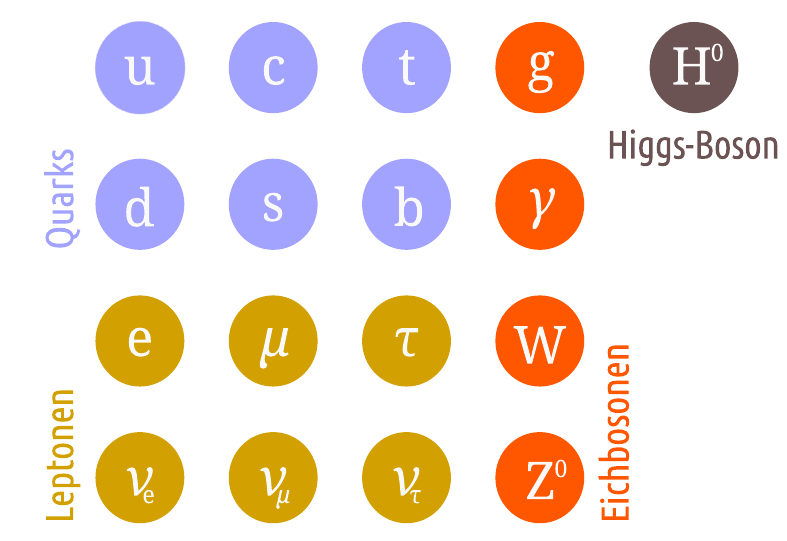
\includegraphics[width=0.47\textwidth]{SM.png}
      \end{figure}
  \end{multicols}
\end{frame}

\begin{frame}[t]{Motivation}
  \begin{itemize}
    \item Im Standardmodell verbotener Zerfall $\text{J}/\psi\rightarrow e^{\pm}\mu^{\mp}$
    \item Suche nach Erweiterungen des Standardmodells
    \item BESIII Analyse [4]: $\mathcal{BR}(\text{J}/\psi\rightarrow e^{\pm}\mu^{\mp})<1.6\cdot 10^{-7}$ (C.L. $\SI{90}{\percent}$)
    \item Bisher keine Analyse mit Daten vom LHCb Detektor
  \end{itemize}
  \ \\
  \ \\
  \begin{framed}
    \centering
    \large{Ziel: Ermittelung einer erwarteten oberen Abschätzung des Verzweigungsverhältnisses}
  \end{framed}
\end{frame}

%------------------------------------------------------------------------------------------
\section{LHCb Detektor}
%------------------------------------------------------------------------------------------
\begin{frame}[t]{LHCb Detektor}
  \begin{figure}
    \centering
    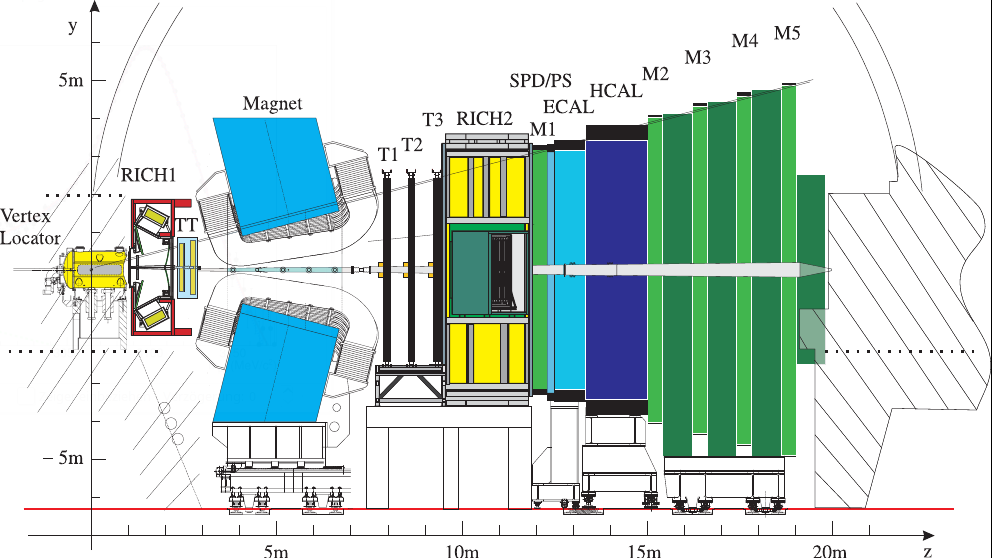
\includegraphics[width=0.76\textwidth]{Detektor.png}[1]
  \end{figure}
\end{frame}

%------------------------------------------------------------------------------------------
\section{Analyse}
%------------------------------------------------------------------------------------------

\begin{frame}
  \begin{block}{Abschätzung Verzweigungsverhältnis}
    \begin{equation*}
      \alpha=N_\text{korr}(\text{J}/\psi)\cdot\frac{\textcolor{blue}{\varepsilon(\text{J}/\psi\rightarrow\mu\mu)}}{\textcolor{red}{\varepsilon(\text{J}/\psi\rightarrow e\mu)}}
    \end{equation*}
    \only<2->{\begin{equation*}
      N_\text{korr}(\text{J}/\psi)=\left(3\frac{\textcolor{blue}{N(\text{J}/\psi\rightarrow \mu\mu)}}{\mathcal{BR}(B^+\rightarrow\text{J}/\psi K^+)\mathcal{BR}(\text{J}/\psi\rightarrow\mu\mu)}+2N(B^0)\frac{f_s}{f_d}\right)^{-1}\frac{1}{\mathcal{BR}(B\rightarrow\text{J}/\psi X)}
    \end{equation*}}
    \only<3->{\begin{equation*}
      \mathcal{BR}(\text{J}/\psi\rightarrow e^{\pm}\mu^{\mp})<\textcolor{red}{N_{\text{J}/\psi\rightarrow e\mu}}\cdot\underbrace{ N_\text{korr}(\text{J}/\psi)\cdot\frac{\textcolor{blue}{\varepsilon(\text{J}/\psi\rightarrow\mu\mu)}}{\textcolor{red}{\varepsilon(\text{J}/\psi\rightarrow e\mu)}}}_{\alpha}
    \end{equation*}}
\end{block}
  \only<1>{Zwischenziel: Bestimmung der Normierungskonstante $\alpha$}
  \only<2>{\begin{itemize}
  \item Diese Analyse:
    \begin{itemize}
      \item Ermittelung der Gesamteffizienz $\textcolor{blue}{\varepsilon(\text{J}/\psi\rightarrow \mu\mu)}$ der Analyse:
        $\varepsilon(\text{J}/\psi\rightarrow \mu\mu)=\varepsilon_\text{geom}\cdot\varepsilon_\text{pre-selection}\cdot\varepsilon_\text{selection}\cdot\varepsilon_\text{trigger}$
      \item Bestimmung der Anzahl der Signalereignisse $\textcolor{blue}{N(\text{J}/\psi\rightarrow \mu\mu)}$ für den Kontrollzerfall $B^+\rightarrow\text{J}/\psi(\rightarrow\mu\mu)K^+$
    \end{itemize}
  \end{itemize}}
  \only<3>{In Kombination mit Ergebnissen aus [5]: Ermittelung der erwarteten oberen Grenze des Verzweigungsverhältnisses $\mathcal{BR}(\text{J}/\psi\rightarrow e^{\pm}\mu^{\mp})$}
\end{frame}

\begin{frame}[t]{Datensatz}
  Bestimmung der Gesamteffizienz der Analyse.
  \begin{itemize} \setlength\itemsep{0.4cm}
    \item Zerfall $B^+\rightarrow\text{J}/\psi(\rightarrow\mu\mu)K^+$
    \item Daten aus dem Jahr 2012
    \item Schwerpunktsenergie $\sqrt{s}=\SI{8}{\tera\electronvolt}$
    \item Integrierte Luminosität $\SI{2}{\femto\barn^{-1}}$
    \item Monte Carlo Simulation
    \item Vorselektion: $\varepsilon_\text{pre-selection}=\SI{8,744(6)}{\percent}$
  \end{itemize}
  \begin{textblock*}{8.5cm}(7cm, 3cm)
    \begin{figure}
      \includegraphics[width=8.5cm]{Psi_MM.pdf}
    \end{figure}
  \end{textblock*}
\end{frame}

\begin{frame}[t]{Selektion der Signalkandidaten des Kontrollkanals}
      \begin{itemize}
        \item \textbf{C}ut \textbf{R}ecursive \textbf{OP}timizer
        \item Selektion für den Zerfall $\text{J}/\psi\rightarrow e^{\pm}\mu^{\mp}$ (Vergleichbarkeit)
      \end{itemize} \pause
      \ \\
      Variablen:
      \begin{enumerate}
        \item Bereich für kombinierte Myonenmasse: \quad $m_{\mu\mu}$ \pause
        \item Rekonstruktion zum Primärvertex: \quad $\mu^{\pm}:\chi_\text{IP}^2$ \pause
        \item Fehlidentifikation der Myonenspuren: \quad $\mu^{\pm}: \text{GhostProb}$ \pause
        \item Erzeugung der $\text{J}/\psi$ als Signal: \quad $\text{J}/\psi: \text{BKGCAT}$ \pause
        \item Übereinstimmung von Impuls und Spur des $\text{J}/\psi$: \quad $\text{J}/\psi: \text{DIRA}$ \pause
      \end{enumerate}
      \begin{framed}
      \centering
        Effizienz dieser Selektion: $\varepsilon_\text{selection}=\SI{82,09(3)}{\percent}$
      \end{framed}
\end{frame}

\begin{frame}[t]{Trigger}
  %Auf die Daten angewandte Triggerstufen (jeweils mit logischem "und" verknüpft)
  \begin{spacing}{0.8}
    \begin{multicols}{2}
      \begin{table}[htb]
        \centering
        \begin{tabular}{l}
          \toprule
          \small{\textbf{L0-Trigger}}                                 \\
          \quad\small{\texttt{L0MuonDecision\_TOS}}              \\
          \quad\small{\texttt{L0HadronDecision\_TOS}}            \\
          \midrule
          \small{\textbf{HLT1-Trigger}}                               \\
          \quad\small{\texttt{Hlt1TrackAllL0Decision\_TOS}}      \\
          \quad\small{\texttt{Hlt1TrackMuonDecision\_TOS}}       \\
          \midrule
          \small{\textbf{HLT2-Trigger}}                               \\
          \quad\small{\texttt{Hlt2Topo2BodyBBDTDecision\_TOS}}   \\
          \quad\small{\texttt{Hlt2Topo3BodyBBDTDecision\_TOS}}   \\
          \quad\small{\texttt{Hlt2Topo4BodyBBDTDecision\_TOS}}   \\
          \quad\small{\texttt{Hlt2TopoMu2BodyBBDTDecision\_TOS}} \\
          \quad\small{\texttt{Hlt2TopoMu3BodyBBDTDecision\_TOS}} \\
          \quad\small{\texttt{Hlt2TopoMu4BodyBBDTDecision\_TOS}} \\
          \bottomrule
        \end{tabular}
      \end{table}
    \columnbreak
    UND-Verknüpfung zwischen den einzelnen Triggerstufen, ODER-Verknüpfung innerhalb einzelner Stufen
    \ \\
    \ \\
    \begin{itemize}
      \item L0-Trigger: Finde Zerfälle mit $K^+$ sowie $\mu^{\pm}$
      \item HLT1-Trigger:
      \item HLT2-Trigger: Finde Zerfälle von $B$-Mesonen
    \end{itemize}
    \begin{framed}
      \centering
      $\varepsilon_\text{trigger}=\SI{74,15(4)}{\percent}$
    \end{framed}
    \end{multicols}
  \end{spacing}
\end{frame}

\begin{frame}[t]{Übersicht aller Teileffizienzen}
  \begin{table}[htb]
    \centering
    \begin{tabular}{lr@{}c@{}l}
      {Selektionsschritt} & \multicolumn{3}{c}{Effizienz} \\
      \toprule
      Geometrie & $\varepsilon_\text{geom}$&=&$\SI{16,099(21)}{\percent}$   \\
      Vorselektion & $\varepsilon_\text{pre-selection}$&=&$\SI{8,744(6)}{\percent}$   \\
      Selektion & $\varepsilon_\text{selection}$&=&$\SI{82,09(3)}{\percent}$   \\
      Trigger & $\varepsilon_\text{trigger}$&=&$\SI{74,15(4)}{\percent}$   \\
      \midrule
      Gesamteffizienz & $\varepsilon(\text{J}/\psi\rightarrow\mu\mu)$&=&$\SI{0,857(1)}{\percent}$   \\
      \bottomrule
    \end{tabular}
  \end{table} \pause
  \centering
  Aus so selektiertem Datensatz Anzahl der Signalkandidaten $B^+\rightarrow\text{J}/\psi(\rightarrow\mu\mu)K^+$ bestimmen
\end{frame}

\begin{frame}[t]{Massenfit}
  \begin{itemize} \setlength\itemsep{0.4cm}
    \item Modell für die Verteilung der rekonstruierten $\text{J}/\psi$-Masse
    \item extended maximum-likelihood-fit (RooFit)
    \item Massenbereich: $[m(\text{J}/\psi)-150\,\text{MeV}/\text{c}^2, m(\text{J}/\psi)+80\,\text{MeV}/\text{c}^2]$
  \end{itemize}
  \ \\
  \begin{itemize} \setlength\itemsep{0.4cm}
    \item Gesamtmodell bestehend aus Signalfunktion und Untergrundfunktion
    \item Skalierungsfaktor $R\approx 13$ (\leadsto Datensatz mit 100\,000 Ereignissen)
  \end{itemize}
\end{frame}

\begin{frame}[t]{Massenfit}
  \vspace{1cm}
  \begin{itemize} \setlength\itemsep{0.5cm}
    \item<1-> Gaußverteilung
    \item<2-> Ausläufer
    \item<3> \leadsto Crystal Ball\\ Funktion
  \end{itemize}
  \begin{textblock*}{11cm}(5cm, 2cm)
    \begin{figure}
      \includegraphics[width=11cm]{Psi_MM.pdf}
    \end{figure}
  \end{textblock*}
  \begin{textblock*}{1cm}(14.2cm, 7.6cm)
    \small{$m_{\mu\mu}$}
  \end{textblock*}
\end{frame}

\begin{frame}[t]{Massenfit}
  \begin{itemize} \setlength\itemsep{0.25cm}
    \item Signalmodell: Double Crystal Ball Funktion
    \begin{itemize}
      \item Gaußsche Verteilung + Potenzfunktion
    \end{itemize}
    \item Untergrundmodell: Exponentialfunktion
    \item Gesamtmodell: Zwei Crystal Ball Funktionen + Exponentieller Untergrund
  \end{itemize}
\end{frame}

\begin{frame}[t]
  \begin{textblock*}{10cm}(2.2cm, 1.1cm)
    \begin{figure}
      \centering
      \includegraphics[width=10cm]{Fitergebnis.pdf}
    \end{figure}
  \end{textblock*}
\end{frame}

\begin{frame}[t]{Fitergebnis}
  \tikzstyle{textnode} = [rectangle, minimum width=2cm, minimum height=0cm, fill=yellow!60!green!70!, text centered, draw=black]
  \tikzstyle{arrow} = [thick,->,>=stealth]
  \begin{figure}
     \begin{tikzpicture}[node distance=2cm]
       \node (n1) [textnode] {Ergebnis des Massenfits: $\tilde{N}(\text{J}/\psi\rightarrow\mu\mu)=99700\,\pm\,334$};
       \node (n2) [textnode, below of=n1,align=center] {Skalierter Wert: $N(\text{J}/\psi\rightarrow\mu\mu)=1\,341\,204\,\pm\,4493$ };
       %\node (n3) [textnode, below of=n2,align=center] {Physikalische Schnitte};
       %\node (n4) [textnode, below of=n3,align=center] {Untergrunddatensatz\\(\num{153701})};
       \draw [arrow] (n1) -- node [anchor=west] {\color{black}{Skalierungsfaktor $R\approx 13$}} (n2);
       %\draw [arrow] (n2) -- node [anchor=west] {\color{red}{-\num{233947}}} (n3);
       %\draw [arrow] (n3) -- node [anchor=west] {\color{red}{-\num{369}}} (n4);
     \end{tikzpicture}
   \end{figure}
\end{frame}

\begin{frame}[t]{Korrektur der bestimmten Signalereignisse}
  \only<1>{\begin{equation*}
    \alpha=N_\mathrm{korr}(\text{J}/\psi)\cdot\frac{\textcolor{blue}{\varepsilon(\text{J}/\psi\rightarrow\mu\mu)}}{\textcolor{red}{\varepsilon(\text{J}/\psi\rightarrow e\mu)}}
  \end{equation*}}

  \only<2->{\begin{itemize}
    \only<2->{\item Gesucht ist die Anzahl der $\text{J}/\psi$ (detached) aus $B$-Zerfällen}
    \only<3->{\item Bestimme zunächst Anzahl der $B^+$ ($\mathcal{BR}$ aus [pdg]):\\
    \begin{equation*}
      N_{B^+}=\frac{N(\text{J}/\psi\rightarrow\mu^{\pm}\mu^{\mp})}{\mathcal{BR}(B^+\rightarrow\text{J}/\psi K^+)\mathcal{BR}(\text{J}/\psi\rightarrow\mu^{\pm}\mu^{\mp})}\cdot\frac{1}{\varepsilon(\text{J}/\psi\rightarrow\mu\mu)}=(2,56\,\pm\,0,08)\cdot10^{12}
    \end{equation*}}
    \only<4->{\item Entspricht der Anzahl der $B^-$-Mesonen}
    \only<5->{\item Wenn $f_u\approx f_d$[cite], so entspricht dies auch der Anzahl der $B^0$}
    \only<6->{\item Unter gleicher Annahme Berechnung der $B_s$ Mesonen:\\
    \begin{equation*} N_{B_s}= N_{B^+}\cdot\frac{f_s}{f_u}\approx N_{B^0}\cdot\frac{f_s}{f_d}=(6,8\,\pm\,0,6)\cdot10^{11}\end{equation*}}
  \end{itemize}}
\end{frame}

\begin{frame}[t]{Korrektur der bestimmten Signalereignisse}
  \begin{itemize} \setlength\itemsep{0.4cm}
    \item Kombination der verschiedenen $B$-Mesonen
    \item $N_\mathrm{korr}(\text{J}/\psi)=(2N_{B^+}+2N_{B_s}+N_{B^0})\cdot\mathcal{BR}(B\rightarrow\text{J}/\psi X)=(9,9\,\pm\,0,4)\cdot10^{10}$
    \item $\mathcal{BR}(B\rightarrow\text{J}/\psi X)=\SI{1,094(32)}{\percent}$ [pdg]
  \end{itemize}
  \begin{block}{Zwischenergebnis}
    \centering
    Korrigierte Anzahl der $\text{J}/\psi$-Mesonen: $N_\mathrm{korr}(\text{J}/\psi)=(9,9\,\pm\,0,4)\cdot10^{10}$
  \end{block}
\end{frame}

\section{Ergebnisse}

\begin{frame}[t]{Berechnung der Normierungskonstante}
  \begin{equation*}
    \alpha=\textcolor{green}{N_\text{korr}(\text{J}/\psi)}\cdot\frac{\textcolor{blue}{\varepsilon(\text{J}/\psi\rightarrow\mu\mu)}}{\textcolor{red}{\varepsilon(\text{J}/\psi\rightarrow e\mu)}}
  \end{equation*}
  \begin{itemize}
    \item Aus parallel durchgeführter Analyse bestimmte Gesamteffizienz: $\textcolor{red}{\varepsilon(\text{J}/\psi\rightarrow e\mu)}=(1,2\,\pm\,0,4)\cdot10^{-6}$
    \item Aus dieser Analyse bestimmte Gesamteffizienz: $\textcolor{blue}{\varepsilon(\text{J}/\psi\rightarrow\mu\mu)}=\SI{0,857(1)}{\percent}$
    \item korrigierte Anzahl der Signalkandidaten: $\textcolor{green}{N_\mathrm{korr}(\text{J}/\psi)}=(9,9\,\pm\,0,4)\cdot10^{10}$
  \end{itemize}
  \begin{block}{Normierungskonstante}
    \centering
    $\alpha=(1,3\,\pm\,0,4)\cdot10^{-5}$
  \end{block}
\end{frame}

\begin{frame}[t]{Berechnung der erwarteten oberen Abschätzung}
  \begin{equation*}
    \mathcal{BR}(\text{J}/\psi\rightarrow e^{\pm}\mu^{\mp})<\textcolor{red}{N_{\text{J}/\psi\rightarrow e\mu}}\cdot\underbrace{ N_\text{korr}(\text{J}/\psi)\cdot\frac{\textcolor{blue}{\varepsilon(\text{J}/\psi\rightarrow\mu\mu)}}{\textcolor{red}{\varepsilon(\text{J}/\psi\rightarrow e\mu)}}}_{\alpha}
  \end{equation*}
  \begin{itemize}
    \item Aus parallel durchgeführter Analyse bestimmte Anzahl der Zerfallskandidaten: $\textcolor{red}{N_{\text{J}/\psi\rightarrow e\mu}}=7\,\pm\,1$
    \item Aus dieser Analyse bestimmte Normierungskonstante: $\alpha=(1,3\,\pm\,0,4)\cdot10^{-5}$
  \end{itemize}
  \begin{block}{Erwartete obere Abschätzung des Verzweigungsverhältnisses}
    \centering
    $\mathcal{BR}(\text{J}/\psi\rightarrow e^{\pm}\mu^{\mp})<(9,2\,\pm\,3,4)\cdot10^{-5}$
  \end{block}
\end{frame}

%-------------------------------------------------------------------------------
\appendix

\begin{frame}
  \centering
  \Huge{\textbf{Backup}}
\end{frame}

\begin{frame}
  \begin{table}[htb]
    \centering
    \caption{Auf den Datensatz angewendete Selektion.}
    \begin{tabular}{lc}
      \toprule
      Selektionsvariable                & Bedingung      \\
      \midrule
      $m_{B}$                           & $\in[\num{5129},\,\num{5429}]$ MeV/c²  \\
      $B^{+}:\chi_{\text{IP}}^2$        & $<\num{25}$  \\
      $B^{+}:\chi_{\text{VD,PV}}^2$     & $>\num{100}$  \\
      $B^{+}:\text{DIRA}$               & $>\num{0.9995}$  \\
      \bottomrule
    \end{tabular}
    \label{tab:bstrip}
  \end{table}
\end{frame}

\begin{frame}[t]{Das Fit-Modell}
  \begin{equation*}
    \text{CB}(x;\alpha ,n,\mu,\sigma,N)=N\cdot
      \begin{cases}
        \mathrm{exp}{\left(-\frac{(x-\mu)^{2}}{2\sigma^{2}}\right)}, &\text{falls }\frac{x-\mu}{\sigma}>-\alpha \\
        A\cdot\left(B-\frac{x-\mu}{\sigma}\right)^{-n}, &\text{falls }\frac{x-\mu}{\sigma }\leq -\alpha
      \end{cases}
  \end{equation*}
  \ \\
  \ \\
  \begin{equation*}
    B(x; c)= \mathrm{e}^{c\cdot x}
  \end{equation*}
  \ \\
  \begin{equation*}
    \mathrm{G}(m_{\mu\mu}; f)=\mathrm{DCB}(m_{\mu\mu};\alpha_1,\alpha_2,\mu,\sigma_1,\sigma_2,n_1,f) + \mathrm{B}(m_{\mu\mu};c)
  \end{equation*}
\end{frame}


\end{document}
